\documentclass[a4paper,12pt]{article}
\usepackage[russian]{babel}
\usepackage[T2A]{fontenc}
\usepackage[utf8]{inputenc}
\usepackage{geometry}
\usepackage{amsmath}
\usepackage{graphicx}
\usepackage{cancel}
\usepackage{float} 
\usepackage{xcolor}
\usepackage{array}
\usepackage{caption}
\usepackage{booktabs}
\usepackage{amssymb}
\usepackage{subcaption}
\usepackage{pgfplots}
\pgfplotsset{compat=1.18}
\usetikzlibrary{arrows.meta, matrix}
\usepackage{capt-of}
\usepackage{multirow}
\usepackage[siunitx]{circuitikz}
\usepackage[bottom]{footmisc}
\usepackage{tcolorbox}
\usepackage{nicematrix}
\usepackage{tikz}
\usetikzlibrary{positioning, arrows.meta}

% --- hyperref ОДИН РАЗ ---
\usepackage{hyperref}
\hypersetup{linktoc=page}
\hypersetup{
	colorlinks=true,
	linkcolor=red,
	citecolor=red,
	urlcolor=red,
	filecolor=red,
}

% --- Содержание ---
\usepackage{tocloft}
\usepackage{etoolbox}
\usepackage{hyperref}
\hypersetup{
	colorlinks=true,
	linkcolor=red,
	citecolor=red,
	urlcolor=red,
}

% Патчим \tableofcontents: текст строк — без ссылок и чёрный
% Это делается через замену \contentsline внутри TOC
\preto\tableofcontents{%
	\begingroup
	% Переопределяем contentsline так, чтобы текст был чёрным без ссылки,
	% а номер страницы — красной ссылкой
	\renewcommand{\contentsline}[4]{%
		\ifnum\pdfstrcmp{##1}{section}=0
		\vskip 4pt{\normalfont\color{black}##2}\nobreak\hfill
		{\normalfont\color{red}\hyperlink{##4}{##3}}\par
		\else\ifnum\pdfstrcmp{##1}{subsection}=0
		\vskip 2pt\hspace{1.5em}{\normalfont\color{black}##2}\nobreak\hfill
		{\normalfont\color{red}\hyperlink{##4}{##3}}\par
		\else
		\vskip 1pt\hspace{3em}{\normalfont\color{black}##2}\nobreak\hfill
		{\normalfont\color{red}\hyperlink{##4}{##3}}\par
		\fi\fi
	}%
}
\appto\tableofcontents{\endgroup}

% tocloft — только для отступов, без переопределения шрифтов
\usepackage{tocloft}

% --- Листинги ---
\usepackage{listings}

\definecolor{codebg}{RGB}{250,250,252}
\definecolor{linenumcolor}{RGB}{150,150,170}
\definecolor{mathblue}{RGB}{30,100,200}
\definecolor{mathorange}{RGB}{200,100,20}
\definecolor{matlabblue}{RGB}{0,0,200}
\definecolor{matlabgreen}{RGB}{30,130,30}
\definecolor{matlaborange}{RGB}{200,80,0}

\lstdefinelanguage{Mathematica}{
	keywords={Plot, Eigenvalues, MatrixExp, RiccatiSolve, IdentityMatrix,
		Inverse, Transpose, Simplify, Eigensystem, StateSpaceModel,
		ControllabilityMatrix, MatrixRank, Export, FileNameJoin,
		NotebookDirectory, ConstantArray, ZeroMatrix, NDSolve,
		Evaluate, LineLegend, Placed, Directive, Opacity, Filling,
		FillingStyle, PlotStyle, PlotLegends, PlotRange, Frame,
		Axes, FrameLabel, GridLines, GridLinesStyle, AspectRatio,
		Style, FontFamily, FontSize, Thick, Dashed, Dotted,
		DotDashed, RGBColor, GrayLevel, LegendLayout, LabelStyle,
		Subscript, Table, Do, Module, Block, If, True, False, Automatic},
	sensitive=true,
	morecomment=[s]{(*}{*)},
	morestring=[b]",
}

\lstdefinestyle{mma}{
	language=Mathematica,
	basicstyle=\ttfamily\small,
	keywordstyle=\color{mathblue}\bfseries,
	commentstyle=\color{linenumcolor}\itshape,
	stringstyle=\color{mathorange},
	numberstyle=\tiny\color{linenumcolor},
	numbers=left,
	numbersep=10pt,
	backgroundcolor=\color{codebg},
	frame=single,
	frameround=tttt,
	framesep=4pt,
	rulecolor=\color{mathblue!40},
	breaklines=true,
	tabsize=4,
	showstringspaces=false,
	captionpos=b,
	xleftmargin=15pt,
	xrightmargin=5pt,
}

\lstdefinestyle{matlab}{
	language=Matlab,
	basicstyle=\ttfamily\small,
	keywordstyle=\color{matlabblue}\bfseries,
	commentstyle=\color{matlabgreen}\itshape,
	stringstyle=\color{matlaborange},
	numberstyle=\tiny\color{linenumcolor},
	numbers=left,
	numbersep=10pt,
	backgroundcolor=\color{codebg},
	frame=single,
	frameround=tttt,
	framesep=4pt,
	rulecolor=\color{matlabblue!30},
	breaklines=true,
	tabsize=4,
	showstringspaces=false,
	captionpos=b,
	xleftmargin=15pt,
	xrightmargin=5pt,
	escapeinside={\%*}{*)},
	morekeywords={cvx_begin,cvx_end,sdp,variable,minimize,maximize},
}

\lstset{style=mma}

\renewcommand{\lstlistingname}{Листинг}
\DeclareCaptionFormat{redlisting}{#1\textcolor{red}{#2}#3}
\captionsetup[lstlisting]{format=redlisting}

\geometry{left=1.5cm, right=2cm, bottom=2cm, top=2cm}
\captionsetup[figure]{name=Рисунок}
\captionsetup[table]{name=Таблица}
\captionsetup{labelsep=endash}


\begin{document}
	
	\begin{titlepage}
		\centering
		
		\vspace*{0.5cm}
		{\small
			Министерство науки и высшего образования Российской Федерации\\[2pt]
			Федеральное государственное автономное образовательное учреждение\\
			высшего образования\\[2pt]
			\textbf{«Национальный исследовательский университет ИТМО»}\\
		}
		
		\vspace{0.8cm}
		\hrule height 0.8pt
		\vspace{0.3cm}
		
		{\large Факультет систем управления и робототехники}
		
		\vspace{0.3cm}
		\hrule height 0.4pt
		\vspace{2.5cm}
		
		{\Huge\bfseries ОТЧЁТ}\\[0.4cm]
		{\LARGE\bfseries о лабораторной работе}\\[0.8cm]
		
		\begin{tcolorbox}[
			colback=gray!4,
			colframe=gray!10,
			boxrule=0.8pt,
			arc=4pt,
			left=12pt, right=12pt, top=8pt, bottom=8pt
			]
			\centering
			{\large По дисциплине:\\[4pt]}
			{\large\bfseries «Теория опимального управления»}\\[10pt]
			{\large Тема:\\[4pt]}
			{\large\bfseries «Поиск минимума с помощью методов статической оптимизации»} \\[10pt]
			{\large Поток: 1.3 \( \) Вариант: 18}
		\end{tcolorbox}
		
		\vspace{3cm}
		
		\begin{minipage}{0.45\textwidth}
			\raggedright
			{\large\bfseries Студент:}\\[4pt]
			Охрименко Е.\,Д.\\
		\end{minipage}
		\hfill
		\begin{minipage}{0.45\textwidth}
			\raggedleft
			{\large\bfseries Преподаватели:}\\[4pt]
			Герасимов Д.Н.\\
			Паромонов А. В.
		\end{minipage}
		
		\vfill
		\vspace{0.4cm}
		{\large Санкт-Петербург, 2026}
	\end{titlepage}
	
	\newpage
	\tableofcontents
	
	\newpage \section{Общее условие}\label{sec:0}
	
	Найдем минимум критерия качества:
	
\begin{equation}
	J(x,u) = 6x^2 + u^2 + 4xu + 3x + 4u - 9
	\label{eq:J}
\end{equation}

Для статической задачи оптимизации.

\begin{figure}[H]
	\centering
	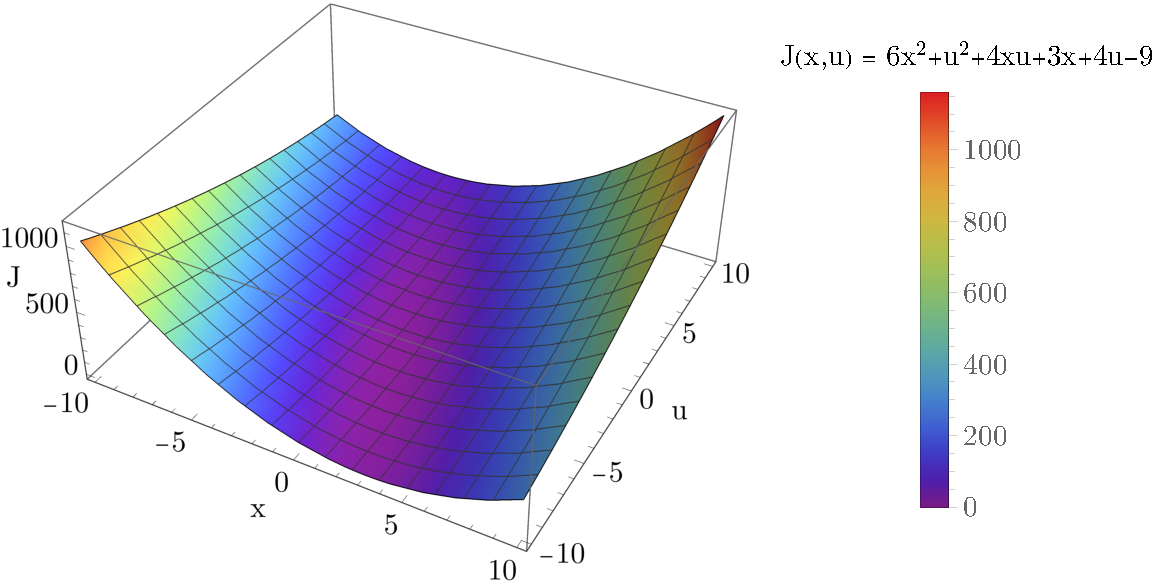
\includegraphics[width=0.8\textwidth]{../images/Jplot.pdf}
	\caption{\(J(x,u)\)}
\end{figure}	
	
	
\newpage \section{Поиск глобального минимума \(J(x,u)\) на основе необходимого и достаточного условий}\label{sec:1}
	
	
\subsection{Без ограничений}	

\[
	J(x,u) = 6x^2 + u^2 + 4xu + 3x + 4u - 9
\]

Проверим необходимое условие минимума. Градиент функционала качества:

\[\begin{aligned}
	\operatorname{grad} J(x,u) = \nabla J(x,u) &= 
	\begin{bmatrix}
		\dfrac{\partial J(x,u)}{\partial x} \\[10pt]
		\dfrac{\partial J(x,u)}{\partial u}
	\end{bmatrix}
	= \begin{bmatrix}
		12x + 4u + 3 \\[10pt]
		2u + 4x + 4
	\end{bmatrix}
    \end{aligned}
\]


Так как:

\[\operatorname{grad} J(x,u) = 0 \qquad \Longrightarrow \qquad
\begin{cases}
	12x + 4u + 3 = 0  \\
	2u + 4x + 4 = 0
\end{cases} \qquad \Longrightarrow \qquad
\begin{cases}
	x^* = \dfrac{5}{4}  \\[10pt]
	u^* = -\dfrac{9}{2}
\end{cases} 
\]

Найдем функционал качества в этой точке:

\[
J^* = J(x^*,u^*) = - 	\dfrac{129}{8}
\]

Проверим достаточное условие минимума. Гессиан функционала качества:	
	
\[
H = \nabla^2 J(x,u) = 
\begin{bmatrix}
	\dfrac{\partial^2 J}{\partial x^2} & \dfrac{\partial^2 J}{\partial x \partial u} \\[8pt]
	\dfrac{\partial^2 J}{\partial u \partial x} & \dfrac{\partial^2 J}{\partial u^2}
\end{bmatrix}
= 
\begin{bmatrix}
	12 & 4 \\
	4 & 2
\end{bmatrix}
\]	
	
Вычислим главные миноры матрицы $H$:
\[
\Delta_1 = 12 > 0, \qquad 
\Delta_2 = \det(H) = 12 \cdot 2 - 4 \cdot 4 = 8 > 0
\]	
	
Так как все главные миноры положительны, матрица $H$ положительно определена. 
Следовательно, точка $(x^*, u^*)$ является точкой глобального минимума.	

\begin{figure}[H]
	\centering
	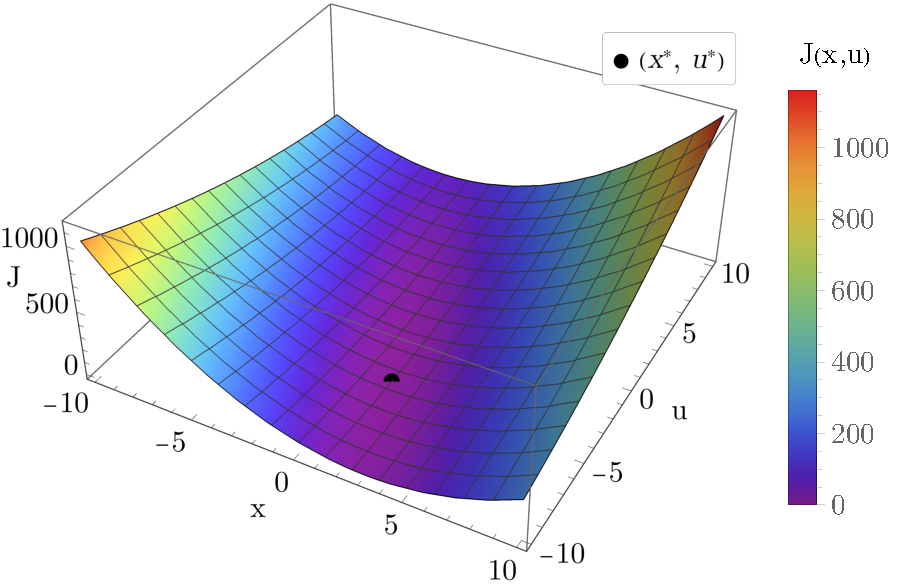
\includegraphics[width=0.6\textwidth]{../images/Jminplot.pdf}
	\caption{\(J(x,u)\) и точка минимума \((x^*,u^*)\)}
\end{figure}	

	
	
\subsection{С ограничением в виде равенства \(c(x,u) = 0\)}	
	
	Рассмотрим функцию:
	
	\[c(x,u) = 3x + 4u^2 + 7\]
	
	Построим лагранжиан:
	
	\[\begin{aligned}
		L( x, u, \lambda) 
		&= J(x, u) + \lambda c(x,u) = 6x^2 + u^2 + 4xu + 3x + 4u - 9 + \lambda (3x + 4u^2 + 7) \\
		&= 6x^2 + (1+4\lambda)u^2 + 4xu + 3x(1+\lambda) + 4u -9 +7 \lambda
	\end{aligned}\]

	Продиффиренцируем по трем переменным:
	
	\[\begin{aligned}
		\dfrac{\partial L}{\partial x} &= 12x + 4u + 3(1+\lambda) \\[5pt]
		\dfrac{\partial L}{\partial u} &= 2u(1+4\lambda) + 4x + 4 \\[5pt]
		\dfrac{\partial L}{\partial \lambda} &= 4u^2 + 3x + 7
	\end{aligned}\]
	
	Приравняем частные производные к нулю и составим систему уравнений:
	
	\[\begin{cases}
		12x + 4u + 3(1+\lambda) = 0 \\[5pt]
		2u(1+4\lambda) + 4x + 4 = 0 \\[5pt]
		4u^2 + 3x + 7 = 0 
	\end{cases}\]
	
Решение нелинейной системы уравнений дает три набора корней. Два из них являются комплексно-сопряженными:

\[
\begin{cases}
	x_{1,2} \approx -0.277 \pm 0.494i \\[5pt]
	u_{1,2} \approx 0.148 \pm 1.251i \\[5pt]
	\lambda_{1,2} \approx -0.089 \pm 0.308i
\end{cases}
\]

Данные решения содержат мнимую часть, поэтому они отбрасываются. Единственным вещественным решением является:

\[
\begin{cases}
	x^* \approx -2.342 \\[5pt]
	u^* \approx 0.0788 \\[5pt]
	\lambda^* \approx 8.261
\end{cases}
\]

Таким образом, стационарная точка задачи: $(x^*, u^*) \approx (-2.342; \, 0.0788)$. Значение критерия качества в этой точке:
\[
J^* = J(x^*, u^*) \approx 15.73
\]
	
	
	
Для построения траектории допустимого множества выразим переменную $x$ из уравнения ограничения $c(x,u)=0$:

\[
3x + 4u^2 + 7 = 0 \quad \Longrightarrow \quad x(u) = -\frac{4u^2 + 7}{3}
\]
	
	
\begin{figure}[H]
	\centering
	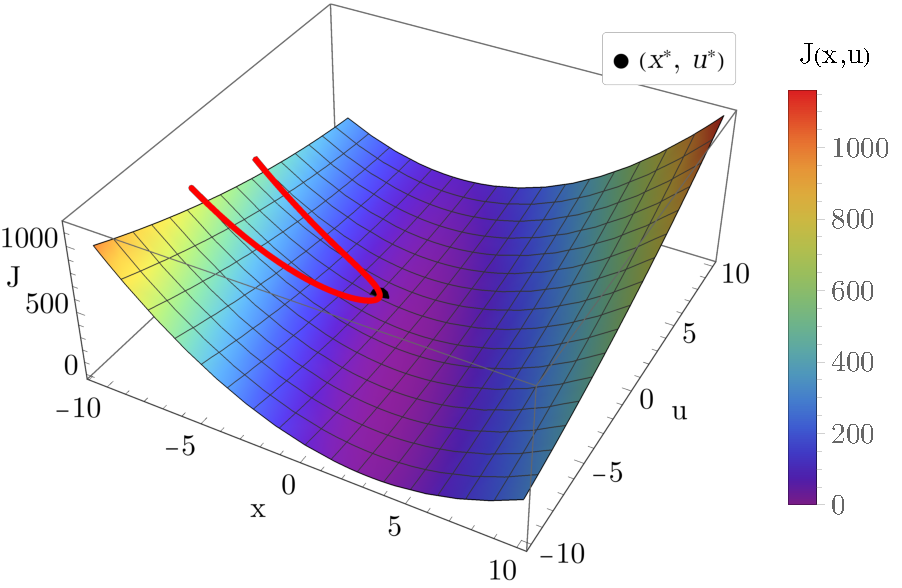
\includegraphics[width=0.6\textwidth]{../images/Jeqplot.pdf}
	\caption{\(J(x,u)\), точка минимума \((x^*,u^*)\) и траектория \(c(x,u)\)}
\end{figure}		
	

	
\subsection{С ограничением в виде неравенства \(c(x,u) \leq 0\)}

Рассмотрим задачу минимизации \(J(x,u)\) при условии:

 \[3x + 4u^2 + 7 \leq 0\]
 
 Согласно теореме Куна-Таккера, необходимые условия экстремума для задачи минимизации при ограничении \(c(x,u) \leq 0\) имеют вид:
 \[
 \begin{cases}
 	\nabla_x L(x, u, \lambda) = 0 \\
 	c(x,u) \leq 0 \\
 	\lambda \geq 0 \\
 	\lambda \cdot c(x,u) = 0
 \end{cases}
 \]

\textit{1. Неактивное ограничение (\(\lambda = 0\)).}
Глобальный минимум не удовлетворяет условию допустимости:
\[
c\left(\dfrac{5}{4}; -\dfrac{9}{2}\right) = 91.75 > 0
\]
Следовательно, этот случай невозможен.

\textit{2. Активное ограничение (\(\lambda > 0, c(x,u) = 0\)).}
Минимум лежит на границе. Система уравнений совпадает с задачей из п. 2.2. Найденное решение удовлетворяет условию неотрицательности множителя:
\[
x^* \approx -2.342 \qquad u^* \approx 0.0788 \qquad \lambda^* \approx 8.261 > 0
\]

Значение критерия качества:
\[
J^* \approx 15.73
\]
	
	
	
\newpage \section{Градиентный поиск минимума критерия качества}	

\subsection{Метод Ньютона-Рафсона}

Для поиска минимума используем итерационную формулу:
\[
x_{k+1} = x_k - H^{-1}(x_k) \nabla J(x_k).
\]

Поскольку \(J(x,u)\) квадратична, Гессиан постоянен:
\[
H = \begin{bmatrix} 12 & 4 \\ 4 & 2 \end{bmatrix} \qquad H^{-1} = \begin{bmatrix} 0.25 & -0.5 \\ -0.5 & 1.5 \end{bmatrix}
\]

При начальном приближении \(x_0 = [0; 0]\) градиент \(\nabla J(x_0) = [3; 4]\). Выполняем одну итерацию \ref{lst:newton}:
\[
x_1 = \begin{bmatrix} 0 \\ 0 \end{bmatrix} - \begin{bmatrix} 0.25 & -0.5 \\ -0.5 & 1.5 \end{bmatrix} \begin{bmatrix} 3 \\ 4 \end{bmatrix} = \begin{bmatrix} 1.25 \\ -4.5 \end{bmatrix}
\]

Сходимость за одну итерацию обусловлена квадратичностью функционала. Результат совпадает с аналитическим решением п. 2.1:
\[
x^* = 1.25 \qquad u^* = -4.5 \qquad J^* = -16.125
\]
	
	

\subsection{Метод наискорейшего спуска}

Итерационная формула имеет вид (Листинг~\ref{lst:grad_descent}):
\[
x_{k+1} = x_k - \gamma \nabla J(x_k)
\]

Выбор шага $\gamma$ эвристический.  Подобраны два значения: $\gamma_1 = 0.05$ (апериодическая сходимость) и $\gamma_2 = 0.12$ (колебательная сходимость). Начальное значение примем:
\[x_0 = [-10, 7]\]

Критерием остановки служит условие:
 \[\|\nabla J(x_k)\| < \text{tol}\]
 где $\text{tol} = 10^{-6}$. 
 
 Максимальное число итераций ограничено 500.

\subsubsection{Апериодическая сходимость}
	При $\gamma_1 = 0.05$ метод не достиг заданной точности за отведенные 500 итераций, что свидетельствует о крайне медленной сходимости при малых значениях шага. Траектория плавно выходит на оптимум.
	
	\begin{figure}[H]
		\centering
		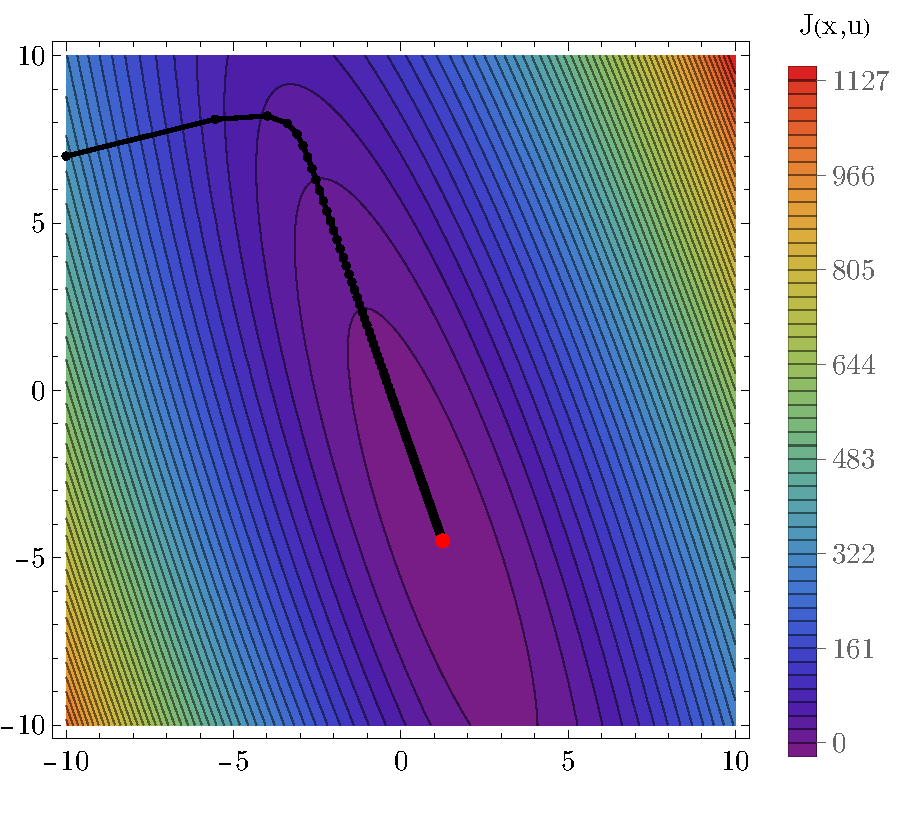
\includegraphics[width=0.6\textwidth]{../images/jGamma005.pdf}
		\caption{Траектория метода наискорейшего спуска при $\gamma = 0.05$}
	\end{figure}
	
	
	\subsubsection{Колебательная сходимость}
	
	
	При $\gamma_2 = 0.12$ траектория колеблется первые несколько шагов. Сходимость была достигнута за 218 итераций, что подтверждает эффективность выбора большего шага для данной задачи.
	
	\begin{figure}[H]
		\centering
		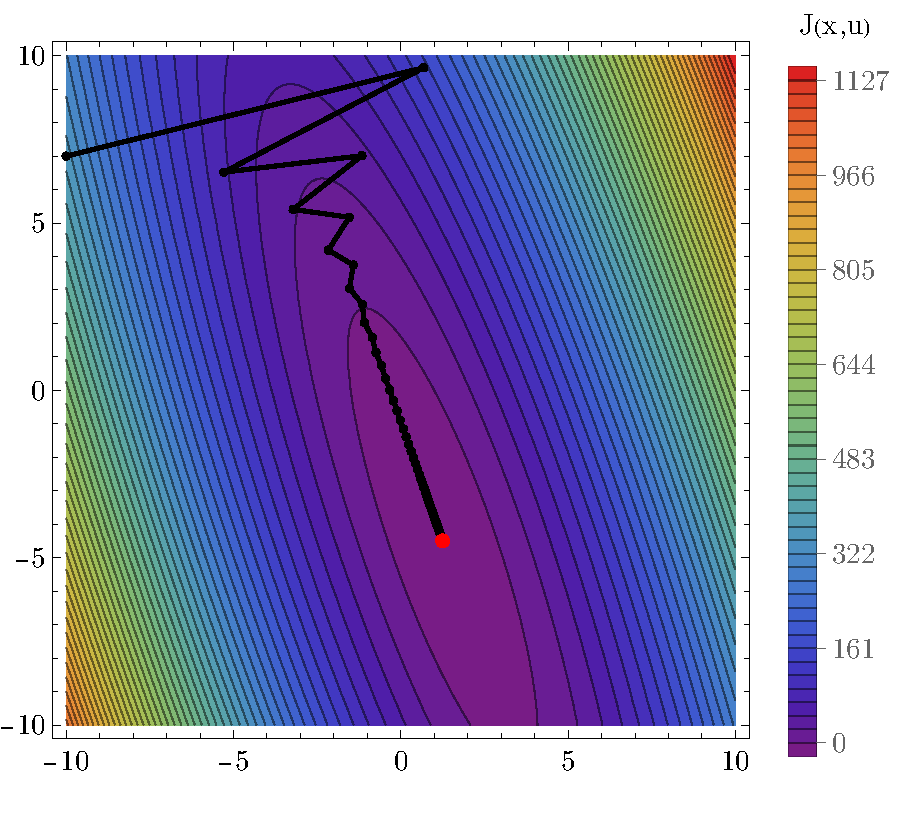
\includegraphics[width=0.6\textwidth]{../images/jGamma012.pdf}
		\caption{Траектория метода наискорейшего спуска при $\gamma = 0.12$}
	\end{figure}

	
	
	\section{Вывод}
	
	В ходе выполнения лабораторной работы был найден безусловный минимум функционала качества $J(x,u)$ аналитически и численно методом Ньютона-Рафсона, который сошёлся за одну итерацию благодаря квадратичности целевой функции. Метод наискорейшего спуска продемонстрировал зависимость характера сходимости от выбора шага $\gamma$: при малом значении ($\gamma=0.05$) наблюдается медленная апериодическая сходимость, не достигшая заданной точности за 500 итераций, тогда как увеличенный шаг ($\gamma=0.12$) обеспечил решение задачи за 218 итераций с характерным колебательным режимом приближения к оптимуму.
	
	
	
	
	
	
	
	
	
	
	
	
	
	
	
	
	
	

	
\newpage
\section{Приложение}

\begin{lstlisting}[caption={Инициализация}, language=matlab]
clc; clear;
syms x u lam
J = 6*x^2 + u^2 + 4*x*u + 3*x + 4*u - 9;
\end{lstlisting}

\begin{lstlisting}[caption={\(J, H\) и оптимальная точка}, language=matlab]
grad_J = jacobian(J, [x, u]);
hess_J = hessian(J, [x, u])

[x_star, u_star] = solve(grad_J == 0, [x, u]);
disp('x*:'); disp(x_star);
disp('u*:'); disp(u_star);

J_min = subs(J, {x, u}, {x_star, u_star})
\end{lstlisting}


\begin{lstlisting}[caption={Решение системы уравнений}, language=matlab]
eq1 = 12*x + 4*u + 3*(1 + lam) == 0;
eq2 = 2*(1 + 4*lam)*u + 4*x + 4 == 0;
eq3 = 4*u^2 + 3*x + 7 == 0;

sol = solve([eq1, eq2, eq3], [x, u, lam]);

disp('x ='); disp(vpa(sol.x, 4));
disp('u ='); disp(vpa(sol.u, 4));
disp('lambda ='); disp(vpa(sol.lam, 4));
\end{lstlisting}



\newpage
\section*{Приложение (Итеративные методы)}
\begin{lstlisting}[caption={Метод Ньютона (без цикла)}, language=matlab, label={lst:newton}]
x0 = [0; 0];
vec = [x; u];

grad_J_num = subs(grad_J, {x, u}, {x0(1), x0(2)})
x_new = x0 - inv(hess_J) * grad_J_num'
\end{lstlisting}

\begin{lstlisting}[caption={Метод наискорейшего спуска}, label={lst:grad_descent}]
J[x_, u_] := 6 x^2 + u^2 + 4 x u + 3 x + 4 u - 9

hessJ = {{12, 4}, {4, 2}};
x0 = {-10, 7};
history = {x0};

gamma = 0.12;

gradNorm = Norm[Grad[J[x, u], {x, u}] /. {x -> x0[[1]], u -> x0[[2]]}];
tol = 10^-6;

i = 1;
While[i <= 500 && gradNorm > tol,
	gradNum = Grad[J[x, u], {x, u}] /. {x -> x0[[1]], u -> x0[[2]]};
	xNew = x0  - gamma *gradNum;
	
	x0 = xNew;
	AppendTo[history, x0];
	
	gradNorm = Norm[gradNum];
	i++
]
\end{lstlisting}
	
\end{document}